\documentclass[tikz,border=4mm]{standalone}

\usepackage{fontspec}
\usepackage{amsmath}
\usepackage{unicode-math}
\usepackage{tikz}

\usetikzlibrary{arrows.meta,calc,positioning}

% Compile with LuaLaTeX or XeLaTeX.
\setmainfont{STIX Two Text}
\setmathfont{STIX Two Math}

\colorlet{mappingcolor}{blue!58!black}
\colorlet{panelcolor}{blue!42!black}

\tikzset{
  interval/.style={black!88, line width=1pt},
  mapping arrow/.style={
    mappingcolor,
    line width=0.8pt,
    -{Latex[length=2.1mm,width=1.5mm]}
  },
  dimension/.style={
    black!65,
    line width=0.6pt,
    {Latex[length=1.7mm,width=1.2mm]}-{Latex[length=1.7mm,width=1.2mm]}
  }
}

\begin{document}

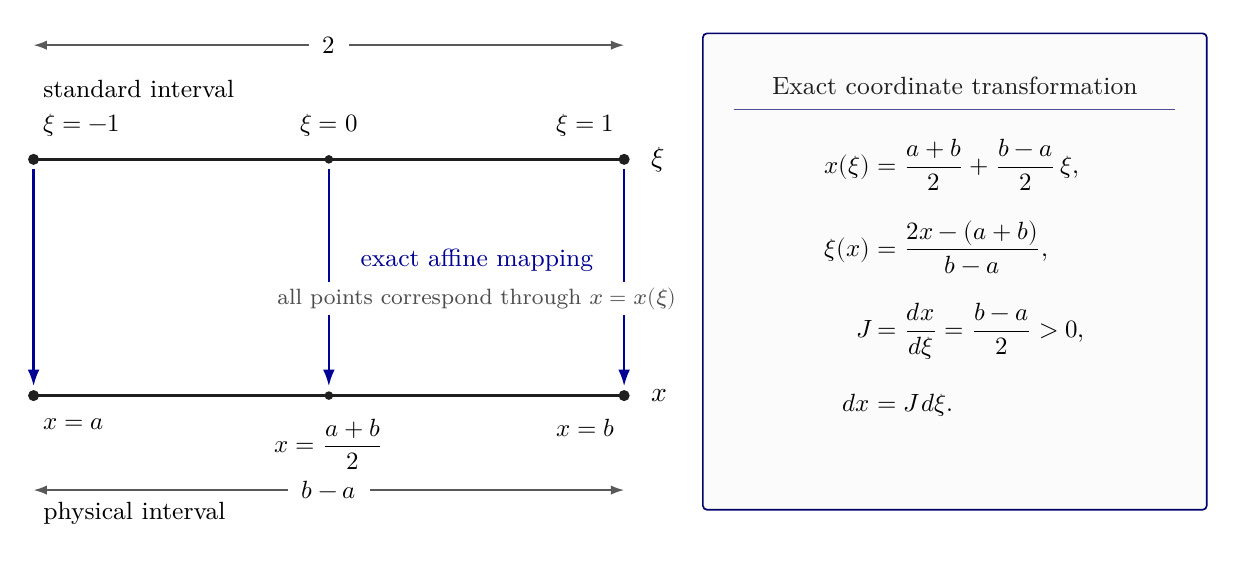
\begin{tikzpicture}[font=\small]

  % Shared schematic positions for the two intervals.
  \coordinate (sL) at (0.25,4.75);
  \coordinate (sM) at (4.00,4.75);
  \coordinate (sR) at (7.75,4.75);
  \coordinate (pL) at (0.25,1.75);
  \coordinate (pM) at (4.00,1.75);
  \coordinate (pR) at (7.75,1.75);

  % Standard interval.
  \node[anchor=west] at (0.25,5.65) {standard interval};
  \draw[interval] (sL) -- (sR);
  \fill[black!88] (sL) circle[radius=2pt];
  \fill[black!88] (sM) circle[radius=1.55pt];
  \fill[black!88] (sR) circle[radius=2pt];
  \node[anchor=south west] at ($(sL)+(0,0.17)$) {$\xi=-1$};
  \node[anchor=south] at ($(sM)+(0,0.17)$) {$\xi=0$};
  \node[anchor=south east] at ($(sR)+(0,0.17)$) {$\xi=1$};
  \node[anchor=west, font=\normalsize] at ($(sR)+(0.22,0)$) {$\xi$};

  % Coordinate length of the standard interval.
  \draw[dimension] (0.25,6.20) -- (7.75,6.20)
    node[midway, fill=white, inner xsep=5pt, text=black] {$2$};

  % Physical interval.
  \draw[interval] (pL) -- (pR);
  \fill[black!88] (pL) circle[radius=2pt];
  \fill[black!88] (pM) circle[radius=1.55pt];
  \fill[black!88] (pR) circle[radius=2pt];
  \node[anchor=north west] at ($(pL)+(0,-0.17)$) {$x=a$};
  \node[anchor=north] at ($(pM)+(0,-0.17)$) {$x=\dfrac{a+b}{2}$};
  \node[anchor=north east] at ($(pR)+(0,-0.17)$) {$x=b$};
  \node[anchor=west, font=\normalsize] at ($(pR)+(0.22,0)$) {$x$};
  \node[anchor=west] at (0.25,0.25) {physical interval};

  % Physical length of the interval.
  \draw[dimension] (0.25,0.55) -- (7.75,0.55)
    node[midway, fill=white, inner xsep=5pt, text=black] {$b-a$};

  % Three representative exact correspondences.  The accompanying note
  % makes explicit that the affine mapping acts on the complete intervals.
  \draw[mapping arrow] ($(sL)+(0,-0.12)$) -- ($(pL)+(0,0.12)$);
  \draw[mapping arrow] ($(sM)+(0,-0.12)$) -- ($(pM)+(0,0.12)$);
  \draw[mapping arrow] ($(sR)+(0,-0.12)$) -- ($(pR)+(0,0.12)$);

  \node[
    align=center,
    text=mappingcolor,
    fill=white,
    inner sep=3pt
  ] at (5.88,3.47) {exact affine mapping};
  \node[
    align=center,
    text=black!70,
    font=\footnotesize,
    fill=white,
    inner sep=2pt
  ] at (5.88,2.98) {all points correspond through $x=x(\xi)$};

  % Formula panel.
  \fill[black!1.5, rounded corners=1.5pt]
    (8.75,0.30) rectangle (15.15,6.35);
  \draw[panelcolor, line width=0.6pt, rounded corners=1.5pt]
    (8.75,0.30) rectangle (15.15,6.35);

  \node[anchor=north, text=black!88] at (11.95,5.92)
    {Exact coordinate transformation};
  \draw[panelcolor!70, line width=0.45pt]
    (9.15,5.38) -- (14.75,5.38);

  \node[align=left] at (11.95,3.22) {$\displaystyle
    \begin{aligned}
      x(\xi)
        &= \frac{a+b}{2}+\frac{b-a}{2}\,\xi, \\[2.4mm]
      \xi(x)
        &= \frac{2x-(a+b)}{b-a}, \\[2.4mm]
      J
        &= \frac{dx}{d\xi}=\frac{b-a}{2}>0, \\[2.4mm]
      dx
        &= J\,d\xi.
    \end{aligned}
  $};

\end{tikzpicture}

\end{document}
